% questions.tex —— 2005 年·普通高等学校招生考试·江西卷·文科 · 题目内容片段（无答案）
% 由 tools/generate_projects.py 依来源总账自 2005/2005_数学真题_江西文科_试题.md 生成，勿手改（改源 MD 后重跑）

\gkpart{一、选择题：本大题共 12 小题，每小题 5 分，共 60 分．在每小题给出的四个选项中，只有一项是符合题目要求的．}

\begin{question}
\gkti{1}设集合 $I = \{x \mid |x| < 3, x \in \mathbf{Z}\}, A = \{1, 2\}, B = \{-2, -1, 2\}$，则 $A \cup (\complement_I B) =$\mbox{（　　）}

\begin{gkopts}(4)
\task A．$\{1\}$
\task B．$\{1, 2\}$
\task C．$\{2\}$
\task D．$\{0, 1, 2\}$
\end{gkopts}

\end{question}
\begin{question}
\gkti{2}已知 $\tan\dfrac{\alpha}{2} = 3$，则 $\cos\alpha =$\mbox{（　　）}

\begin{gkopts}(4)
\task A．$\dfrac{4}{5}$
\task B．$-\dfrac{4}{5}$
\task C．$\dfrac{4}{15}$
\task D．$-\dfrac{3}{5}$
\end{gkopts}

\end{question}
\begin{question}
\gkti{3}$(\sqrt{x} + \sqrt[3]{x})^{12}$ 的展开式中，含 $x$ 的正整数次幂的项共有\mbox{（　　）}

\begin{gkopts}(4)
\task A．4 项
\task B．3 项
\task C．2 项
\task D．1 项
\end{gkopts}

\end{question}
\begin{question}
\gkti{4}函数 $f(x) = \dfrac{1}{\log_2(-x^2 + 4x - 3)}$ 的定义域为\mbox{（　　）}

\begin{gkopts}(2)
\task A．$(1, 2) \cup (2, 3)$
\task B．$(-\infty, 1) \cup (3, +\infty)$
\task C．$(1, 3)$
\task D．$[1, 3]$
\end{gkopts}

\end{question}
\begin{question}
\gkti{5}设函数 $f(x) = \sin 3x + |\sin 3x|$，则 $f(x)$ 为\mbox{（　　）}

\begin{gkopts}(2)
\task A．周期函数，最小正周期为 $\dfrac{\pi}{3}$
\task B．周期函数，最小正周期为 $\dfrac{2\pi}{3}$
\task C．周期函数，最小正周期为 $2\pi$
\task D．非周期函数
\end{gkopts}

\end{question}
\begin{question}
\gkti{6}已知向量 $\vec{a} = (1, 2), \vec{b} = (-2, -4), |\vec{c}| = \sqrt{5}$，若 $(\vec{a} + \vec{b}) \cdot \vec{c} = \dfrac{5}{2}$，则 $\vec{a}$ 与 $\vec{c}$ 的夹角为\mbox{（　　）}

\begin{gkopts}(4)
\task A．$30^\circ$
\task B．$60^\circ$
\task C．$120^\circ$
\task D．$150^\circ$
\end{gkopts}

\end{question}
\begin{question}
\gkti{7}将 9 个人（含甲、乙）平均分成三组，甲、乙分在同一组，则不同分组方法的种数为\mbox{（　　）}

\begin{gkopts}(4)
\task A．70
\task B．140
\task C．280
\task D．840
\end{gkopts}

\end{question}
\begin{question}
\gkti{8}在 $\triangle ABC$ 中，设命题 $p: \dfrac{a}{\sin B} = \dfrac{b}{\sin C} = \dfrac{c}{\sin A}$，命题 $q: \triangle ABC$ 是等边三角形，那么命题 $p$ 是命题 $q$ 的\mbox{（　　）}

\begin{gkopts}(2)
\task A．充分不必要条件
\task B．必要不充分条件
\task C．充分必要条件
\task D．既不充分又不必要条件
\end{gkopts}

\end{question}
\begin{question}
\gkti{9}矩形 $ABCD$ 中，$AB = 4, BC = 3$，沿 $AC$ 将矩形 $ABCD$ 折成一个直二面角 $B - AC - D$，则四面体 $ABCD$ 的外接球的体积为\mbox{（　　）}

\begin{gkopts}(2)
\task A．$\dfrac{125}{12}\pi$
\task B．$\dfrac{125}{9}\pi$
\task C．$\dfrac{125}{6}\pi$
\task D．$\dfrac{125}{3}\pi$
\end{gkopts}

\end{question}
\begin{question}
\gkti{10}已知实数 $a, b$ 满足等式 $\left(\dfrac{1}{2}\right)^a = \left(\dfrac{1}{3}\right)^b$，下列五个关系式：
① $0 < b < a$；② $a < b < 0$；③ $0 < a < b$；④ $b < a < 0$；⑤ $a = b$．
其中不可能成立的关系式有\mbox{（　　）}

\begin{gkopts}(4)
\task A．1 个
\task B．2 个
\task C．3 个
\task D．4 个
\end{gkopts}

\end{question}
\begin{question}
\gkti{11}在 $\triangle OAB$ 中，$O$ 为坐标原点，$A(1, \cos\theta), B(\sin\theta, 1), \theta \in \left(0, \dfrac{\pi}{2}\right]$，则 $\triangle OAB$ 的面积达到最大值时，$\theta =$\mbox{（　　）}

\begin{gkopts}(4)
\task A．$\dfrac{\pi}{6}$
\task B．$\dfrac{\pi}{4}$
\task C．$\dfrac{\pi}{3}$
\task D．$\dfrac{\pi}{2}$
\end{gkopts}

\Needspace{0.4\textheight}
\end{question}
\begin{question}
\gkti{12}为了解某校高三学生的视力情况，随机地抽查了该校 100 名高三学生的视力情况，得到频率分布直方图．由于不慎将部分数据丢失，但知道前 4 组的频数成等比数列，后 6 组的频数成等差数列，设最大频率为 $a$，视力在 4.6 到 5.0 之间的学生数为 $b$，则 $a, b$ 的值分别为\mbox{（　　）}

\begin{gkopts}(4)
\task A．$0.27, 78$
\task B．$0.27, 83$
\task C．$2.7, 78$
\task D．$2.7, 83$
\end{gkopts}
\nopagebreak[4]
\begin{center}\begin{tikzpicture}[x=1.2cm,y=1.2cm,>=stealth]
  % 坐标轴
  \draw[->] (0,0) -- (10.5,0) node[above right] {视力};
  \draw[->] (0,0) -- (0,3.3) node[above right] {$\dfrac{\text{频率}}{\text{组距}}$};
  \node[below left] at (0,0) {$0$};

  % 截断标记 (break)
  \draw[thick] (0.35,-0.08) -- (0.45,0.08) -- (0.55,-0.08) -- (0.65,0.08);

  % 横轴刻度与标签
  \foreach \x/\val in {1/4.3, 2/4.4, 3/4.5, 4/4.6, 5/4.7, 6/4.8, 7/4.9, 8/5.0, 9/5.1, 10/5.2} {
    \draw (\x,0) -- (\x,-0.08) node[below] {\small \val};
  }

  % 直方图矩形 (高度为 频率/组距)
  % [4.3, 4.4]: 0.1
  \draw[thick] (1,0) rectangle (2,0.1);
  % [4.4, 4.5]: 0.3
  \draw[thick] (2,0) rectangle (3,0.3);
  % [4.5, 4.6]: 0.9
  \draw[thick] (3,0) rectangle (4,0.9);
  % [4.6, 4.7]: 2.7 (最大频率 0.27)
  \draw[thick] (4,0) rectangle (5,2.7);
  % [4.7, 4.8]: 2.2
  \draw[thick] (5,0) rectangle (6,2.2);
  % [4.8, 4.9]: 1.7
  \draw[thick] (6,0) rectangle (7,1.7);
  % [4.9, 5.0]: 1.2
  \draw[thick] (7,0) rectangle (8,1.2);
  % [5.0, 5.1]: 0.7
  \draw[thick] (8,0) rectangle (9,0.7);
  % [5.1, 5.2]: 0.2
  \draw[thick] (9,0) rectangle (10,0.2);

  % 纵轴刻度与虚线辅助线
  \draw (0,0.1) -- (-0.08,0.1) node[left] {\small $0.1$};
  \draw[dashed] (0,0.1) -- (1,0.1);

  \draw (0,0.3) -- (-0.08,0.3) node[left] {\small $0.3$};
  \draw[dashed] (0,0.3) -- (2,0.3);
\end{tikzpicture}
\end{center}
\nopagebreak[4]
\end{question}
\gkpart{二、填空题：本大题共 4 小题，每小题 4 分，共 16 分．把答案填在题中横线上．}

\begin{question}
\gkti{13}若函数 $f(x) = \log_a(x + \sqrt{x^2 + 2a^2})$ 是奇函数，则 $a = \underline{\hspace{2em}}$．

\end{question}
\begin{question}
\gkti{14}设实数 $x, y$ 满足 $\begin{cases} x - y - 2 \leqslant 0, \\ x + 2y - 4 > 0, \\ 2y - 3 \leqslant 0, \end{cases}$ 则 $\dfrac{y}{x}$ 的最大值是 $\underline{\hspace{2em}}$．

\Needspace{0.4\textheight}
\end{question}
\begin{question}
\gkti{15}如图，在三棱锥 $P - ABC$ 中，$PA = PB = PC = BC$，且 $\angle BAC = \dfrac{\pi}{2}$，则 $PA$ 与底面 $ABC$ 所成角为 $\underline{\hspace{2em}}$．
\nopagebreak[4]
\begin{center}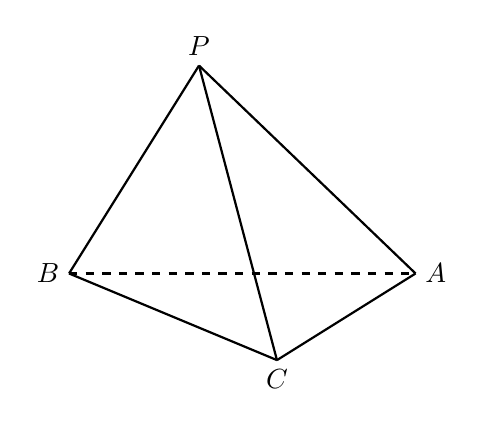
\begin{tikzpicture}[scale=1.1,>=stealth]
  % 顶点坐标
  \coordinate (P) at (1.5, 3.2);
  \coordinate (B) at (0, 0.8);
  \coordinate (A) at (4.0, 0.8);
  \coordinate (C) at (2.4, -0.2);

  % 棱
  \draw[thick] (P) -- (B);
  \draw[thick] (P) -- (C);
  \draw[thick] (P) -- (A);
  \draw[thick] (B) -- (C);
  \draw[thick] (C) -- (A);
  \draw[dashed, thick] (B) -- (A);

  % 顶点标注
  \node[above] at (P) {$P$};
  \node[left] at (B) {$B$};
  \node[below] at (C) {$C$};
  \node[right] at (A) {$A$};
\end{tikzpicture}
\end{center}
\nopagebreak[4]
\end{question}
\begin{question}
\gkti{16}以下四个关于圆锥曲线的命题中：
① 设 $A, B$ 为两个定点，$k$ 为非零常数，$||\vec{PA}| - |\vec{PB}|| = k$，则动点 $P$ 的轨迹为双曲线；
② 设定圆 $C$ 上一定点 $A$ 作圆的动点弦 $AB$，$O$ 为坐标原点，若 $\vec{OP} = \dfrac{1}{2}(\vec{OA} + \vec{OB})$，则动点 $P$ 的轨迹为椭圆；
③ 方程 $2x^2 - 5x + 2 = 0$ 的两根可分别作为椭圆和双曲线的离心率；
④ 双曲线 $\dfrac{x^2}{25} - \dfrac{y^2}{9} = 1$ 与椭圆 $\dfrac{x^2}{35} + y^2 = 1$ 有相同的焦点．
其中真命题的序号为 $\underline{\hspace{2em}}$．（写出所有真命题的序号）

\end{question}
\gkpart{三、解答题：本大题共 6 小题，共 74 分．解答应写出文字说明、证明过程或演算步骤．}

\begin{question}
\gkti{17}已知函数 $f(x) = \dfrac{x^2}{ax + b}$（$a, b$ 为常数），且方程 $f(x) - x + 12 = 0$ 有两个实根为 $x_1 = 3, x_2 = 4$．
(1) 求函数 $f(x)$ 的解析式；
(2) 设 $k > 1$，解关于 $x$ 的不等式：$f(x) < \dfrac{(k+1)x - k}{2-x}$．

\end{question}
\begin{question}
\gkti{18}已知向量 $\vec{a} = \left(2\cos\dfrac{x}{2}, \tan\left(\dfrac{x}{2} + \dfrac{\pi}{4}\right)\right)$，$\vec{b} = \left(\sqrt{2}\sin\left(\dfrac{x}{2} + \dfrac{\pi}{4}\right), \tan\left(\dfrac{x}{2} - \dfrac{\pi}{4}\right)\right)$，令 $f(x) = \vec{a} \cdot \vec{b}$．求函数 $f(x)$ 的最大值，最小正周期，并写出 $f(x)$ 在 $[0, \pi]$ 上的单调区间．

\end{question}
\begin{question}
\gkti{19}A、B 两位同学各有五张卡片，现以投掷均匀硬币的形式进行游戏，当出现正面朝上时 A 赢得 B 一张卡片，否则 B 赢得 A 一张卡片，如果某人已赢得所有卡片，则游戏终止．求掷硬币的次数不大于 7 次时游戏终止的概率．

\Needspace{0.4\textheight}
\end{question}
\begin{question}
\gkti{20}如图，在长方体 $ABCD - A_1B_1C_1D_1$ 中，$AD = AA_1 = 1, AB = 2$，点 $E$ 在棱 $AB$ 上移动．
(1) 证明：$D_1E \perp A_1D$；
(2) 当 $E$ 为 $AB$ 的中点时，求点 $E$ 到面 $ACD_1$ 的距离；
(3) $AE$ 等于何值时，二面角 $D_1 - EC - D$ 的大小为 $\dfrac{\pi}{4}$．
\nopagebreak[4]
\begin{center}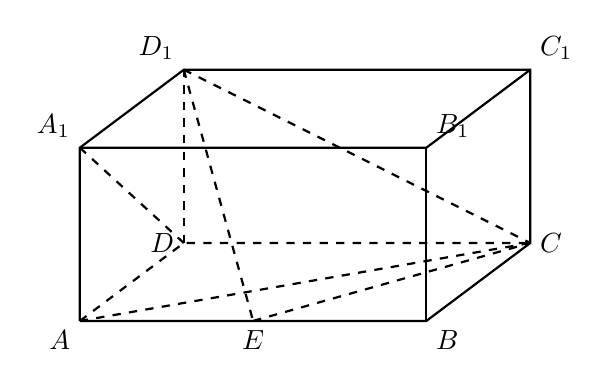
\begin{tikzpicture}[scale=1.1,>=stealth]
  % 顶点坐标
  \coordinate (A) at (0, 0);
  \coordinate (B) at (4.0, 0);
  \coordinate (D) at (1.2, 0.9);
  \coordinate (C) at (5.2, 0.9);

  \coordinate (A1) at (0, 2.0);
  \coordinate (B1) at (4.0, 2.0);
  \coordinate (D1) at (1.2, 2.9);
  \coordinate (C1) at (5.2, 2.9);

  % 点 E 位于 AB 上
  \coordinate (E) at (2.0, 0);

  % 长方体可见棱
  \draw[thick] (A) -- (B) -- (C) -- (C1) -- (D1) -- (A1) -- (A);
  \draw[thick] (A1) -- (B1) -- (C1);
  \draw[thick] (B) -- (B1);

  % 长方体内部不可见棱 (虚线)
  \draw[dashed, thick] (A) -- (D) -- (C);
  \draw[dashed, thick] (D) -- (D1);

  % 辅助线与线段 (虚线)
  \draw[dashed, thick] (D1) -- (E);
  \draw[dashed, thick] (E) -- (C);
  \draw[dashed, thick] (D1) -- (C);
  \draw[dashed, thick] (A) -- (C);
  \draw[dashed, thick] (A1) -- (D);

  % 顶点标签
  \node[below left] at (A) {$A$};
  \node[below right] at (B) {$B$};
  \node[right] at (C) {$C$};
  \node[left] at (D) {$D$};
  \node[above left] at (A1) {$A_1$};
  \node[above right] at (B1) {$B_1$};
  \node[above right] at (C1) {$C_1$};
  \node[above left] at (D1) {$D_1$};
  \node[below] at (E) {$E$};
\end{tikzpicture}
\end{center}
\nopagebreak[4]
\Needspace{0.4\textheight}
\end{question}
\begin{question}
\gkti{21}如图，$M$ 是抛物线 $y^2 = x$ 上的一点，动弦 $ME, MF$ 分别交 $x$ 轴于 $A, B$ 两点，且 $MA = MB$．
(1) 若 $M$ 为定点，证明：直线 $EF$ 的斜率为定值；
(2) 若 $M$ 为动点，且 $\angle EMF = 90^\circ$，求 $\triangle EMF$ 的重心 $G$ 的轨迹方程．
\nopagebreak[4]
\begin{center}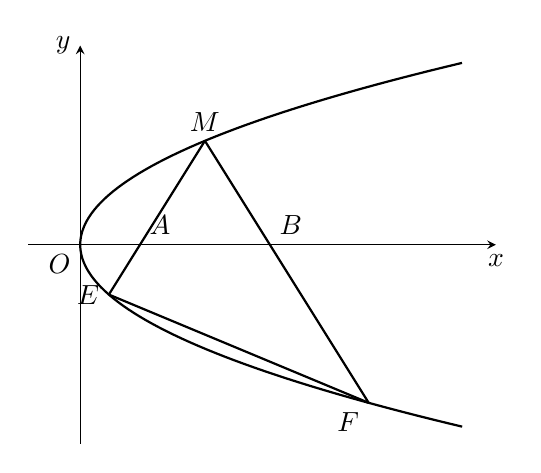
\begin{tikzpicture}[x=1.1cm,y=1.1cm,>=stealth]
  % 坐标轴
  \draw[->] (-0.6,0) -- (4.8,0) node[below] {$x$};
  \draw[->] (0,-2.3) -- (0,2.3) node[left] {$y$};
  \node[below left] at (0,0) {$O$};

  % 抛物线 y^2 = x (即 x = y^2)
  \draw[thick,domain=-2.1:2.1,samples=100] plot ({\x*\x},{\x});

  % 点 M(1.44, 1.2)
  \coordinate (M) at (1.44, 1.2);

  % 动弦 ME, MF
  % 设 k1 = 1.6, k2 = -1.6
  % yE = 1/1.6 - 1.2 = 0.625 - 1.2 = -0.575 => xE = 0.331
  % yF = -1/1.6 - 1.2 = -0.625 - 1.2 = -1.825 => xF = 3.331
  % xA = 1.44 - 1.2/1.6 = 1.44 - 0.75 = 0.69
  % xB = 1.44 + 0.75 = 2.19
  \coordinate (A) at (0.69, 0);
  \coordinate (B) at (2.19, 0);
  \coordinate (E) at (0.331, -0.575);
  \coordinate (F) at (3.331, -1.825);

  % 连线 ME, MF, EF
  \draw[thick] (M) -- (E);
  \draw[thick] (M) -- (F);
  \draw[thick] (E) -- (F);

  % 顶点与点标注
  \node[above] at (M) {$M$};
  \node[above right] at (A) {$A$};
  \node[above right] at (B) {$B$};
  \node[left] at (E) {$E$};
  \node[below left] at (F) {$F$};
\end{tikzpicture}
\end{center}
\nopagebreak[4]
\end{question}
\begin{question}
\gkti{22}已知数列 $\{a_n\}$ 的前 $n$ 项和 $S_n$ 满足 $S_n - S_{n-2} = 3\left(-\dfrac{1}{2}\right)^{n-1}\ (n \geqslant 3)$，且 $S_1 = 1, S_2 = -\dfrac{3}{2}$，求数列 $\{a_n\}$ 的通项公式．

\end{question}